\message{ !name(presentation.tex)}\documentclass[usenames,dvipsnames]{beamer}

\mode<presentation>
{
  \usetheme{CambridgeUS}
  \usecolortheme{orchid}
  \setbeamercovered{transparent}
  \useinnertheme{rectangles}
  \setbeamertemplate{navigation symbols}{}
  \usefonttheme[onlymath]{serif}
  \setbeamercolor{title}{bg=alerted text.fg!85!black, fg=white}
  \setbeamercolor{item projected}{bg=alerted text.fg!85!black}
  \setbeamertemplate{enumerate items}[default]
  \setbeamercolor{local structure}{fg=alerted text.fg!85!black}
  %\setbeamersize{text margin left=0.2cm,text margin right=0.2cm}
}

\newcommand\Shorter[2][1]{%
\makebox[\linewidth][c]{%
  \begin{minipage}{\dimexpr\textwidth+#1\relax}
  \raggedright#2
  \end{minipage}%
  }%
}
\usepackage[english]{babel}
\usepackage[utf8]{inputenc}
\usepackage[T1]{fontenc}
\usepackage{lmodern}
\usepackage{pifont}
\usepackage{mathrsfs}
\usepackage{amsmath}
\usepackage{bm}
\usepackage{caption}
\usepackage{subcaption}
\usepackage{outlines}
\usepackage{booktabs}
\usepackage{anyfontsize}
\usepackage{dirtree}
\usepackage{minted}
\usepackage[listings, minted]{tcolorbox}
\tcbset{left=6mm}
\usepackage[%
autocite     = plain,
doi          = true,
url          = true,
giveninits   = true,
hyperref     = true,
backref      = true,
maxbibnames  = 99,
maxcitenames = 99,
sortcites    = true,
style        = authoryear,
]{biblatex}

\addbibresource{presentation.bib}

\newcommand{\fakeimage}{{\fboxsep=-\fboxrule\fbox{\rule{0pt}{3cm}\hspace{4cm}}}}
\renewcommand*\DTstyle{\textnormal}

\usepackage{tikz}
\usetikzlibrary{quotes}
\usetikzlibrary{bayesnet}
\usetikzlibrary{arrows,calc,positioning,decorations.pathreplacing}
\tikzset{
  >=stealth',
  punkt/.style={
    circle,
    draw=black, thick,
    minimum height=1.75em,
    inner sep=0pt,
    text centered},
  pil/.style={
    ->,
    thick}
}

\definecolor{isabelline}{rgb}{0.96, 0.94, 0.93}
\definecolor{palesilver}{rgb}{0.79, 0.75, 0.73}
\definecolor{hdblue}{HTML}{3366cc}
\hypersetup{colorlinks,linkcolor=,urlcolor=hdblue, citecolor=hdblue}

\setminted{highlightcolor=black!5, linenos}
\setminted{style=emacs}
\setminted{bgcolor=isabelline}
\setminted{fontsize=\fontsize{4.5}{1}\selectfont}
\setminted{highlightcolor=palesilver}
\renewcommand{\theFancyVerbLine}{{\fontsize{4}{1}\selectfont \arabic{FancyVerbLine}}}

\newcommand{\xmark}{\ding{55}}
\newcommand{\highlight}[1]{%
  \colorbox{blue!20}{$\displaystyle#1$}}


\def\ci{\perp\!\!\!\perp}
\makeatletter
\newcommand*{\indep}{%
  \mathbin{%
    \mathpalette{\@indep}{}%
  }%
}
\newcommand*{\nindep}{%
\mathbin{%                   % The final symbol is a binary math operator
  \mathpalette{\@indep}{\not}% \mathpalette helps for the adaptation
  % of the symbol to the different math styles.
}%
}
\def\layersep{.38cm}
\def\inlsep{.4}
\newcommand*{\@indep}[2]{%
% #1: math style
% #2: empty or \not
  \sbox0{$#1\perp\m@th$}%        box 0 contains \perp symbol
  \sbox2{$#1=$}%                 box 2 for the height of =
  \sbox4{$#1\vcenter{}$}%        box 4 for the height of the math axis
  \rlap{\copy0}%                 first \perp
  \dimen@=\dimexpr\ht2-\ht4-.2pt\relax
  % The equals symbol is centered around the math axis.
  % The following equations are used to calculate the
  % right shift of the second \perp:
  % [1] ht(equals) - ht(math_axis) = line_width + 0.5 gap
  % [2] right_shift(second_perp) = line_width + gap
  % The line width is approximated by the default line width of 0.4pt
  \kern\dimen@
  {#2}%
  % {\not} in case of \nindep;
  % the braces convert the relational symbol \not to an ordinary
  % math object without additional horizontal spacing.
  \kern\dimen@
  \copy0 %                       second \perp
}
\makeatother


\title[SCNN]{Predicting Cancer Outcomes from Histology and Genomics Using Convolutional Networks}

% \subtitle
% {Presentation Subtitle} % (optional)

\author[Dogan]
{%
\texorpdfstring{
  \begin{columns}
    \column{.85\linewidth}
    \centering
    Presented by:\\
    Haluk Dogan\\
    \url{https://haluk.github.io/}\\
    \href{mailto:hdogan@vivaldi.net}{hdogan@vivaldi.net} \\
  \end{columns}
}
{Dogan}
}
\institute[SBBI {\fontsize{5}{6}\selectfont @} CSE {\fontsize{5}{6}\selectfont
  @} UNL] % (optional, but mostly needed)
{
  Department of Computer Science\\
  University of Nebraska-Lincoln
}

\date[\today] % (optional)
{\today}

\subject{Talks}

\pgfdeclareimage[height=0.5cm]{university-logo}{figures/logo}
\logo{\pgfuseimage{university-logo}}

\begin{document}

\message{ !name(presentation.tex) !offset(-3) }


\begin{frame}[noframenumbering,plain]
  \titlepage{}
\end{frame}

\section{Introduction}\label{sec:introduction}
\begin{frame}
  \frametitle{Histology}
  \begin{columns}[t]
    \begin{column}{.48\textwidth}
      \vspace{-0.8cm}
      \begin{figure}[ht]
        \centering
        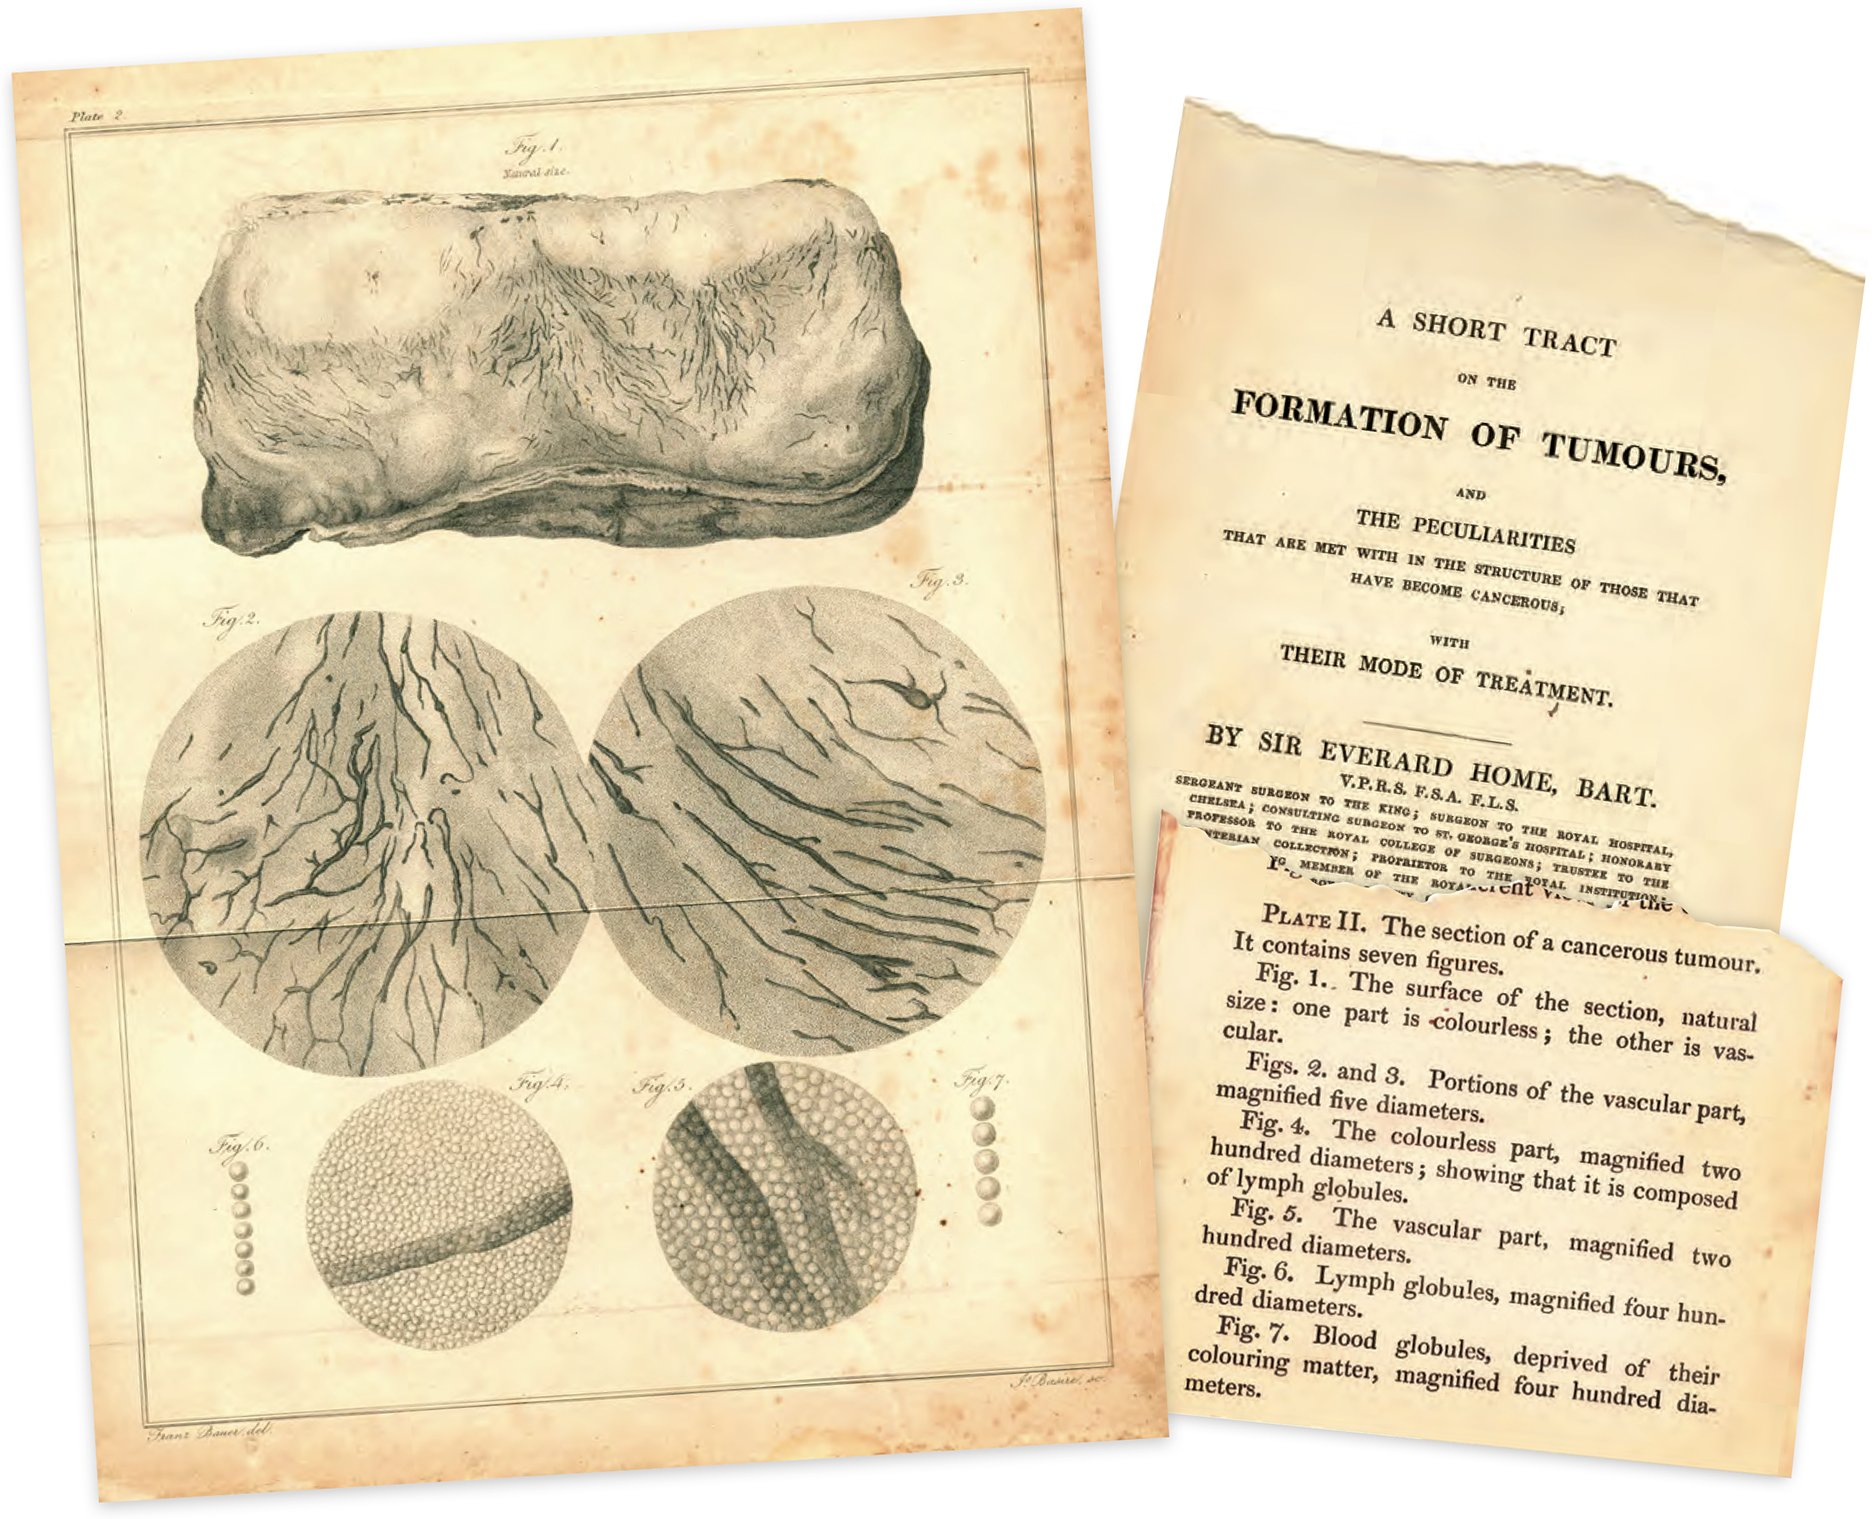
\includegraphics[width=1.0\textwidth,height=0.7\textheight]{figures/early_histology.jpg}
        \caption*{Everard Home in 1830\label{fig:early-histology}}
      \end{figure}
    \end{column}
    \begin{column}{.48\textwidth}
      \vspace{-0.5cm}
      \begin{figure}[ht]
        \centering
        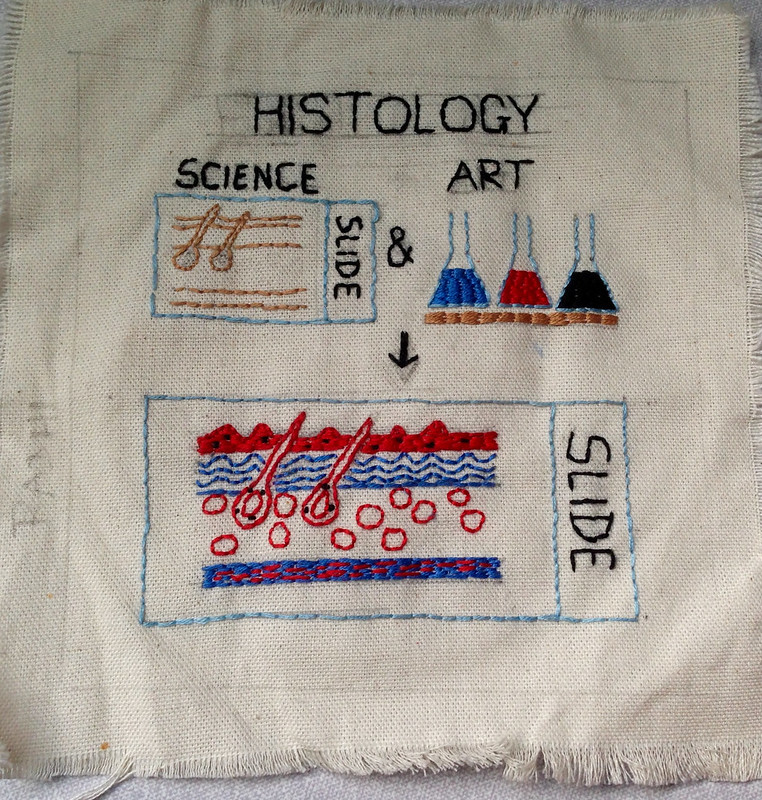
\includegraphics[width=1.0\textwidth,keepaspectratio]{figures/histology_art.jpg}
        \caption*{Science Meets Art\label{fig:histology-art}}
      \end{figure}
    \end{column}
  \end{columns}
\end{frame}
\begin{frame}
  \frametitle{Histology (cont'd)}
  %\vspace{-0.7cm}
  \begin{figure}[ht]
    \centering
    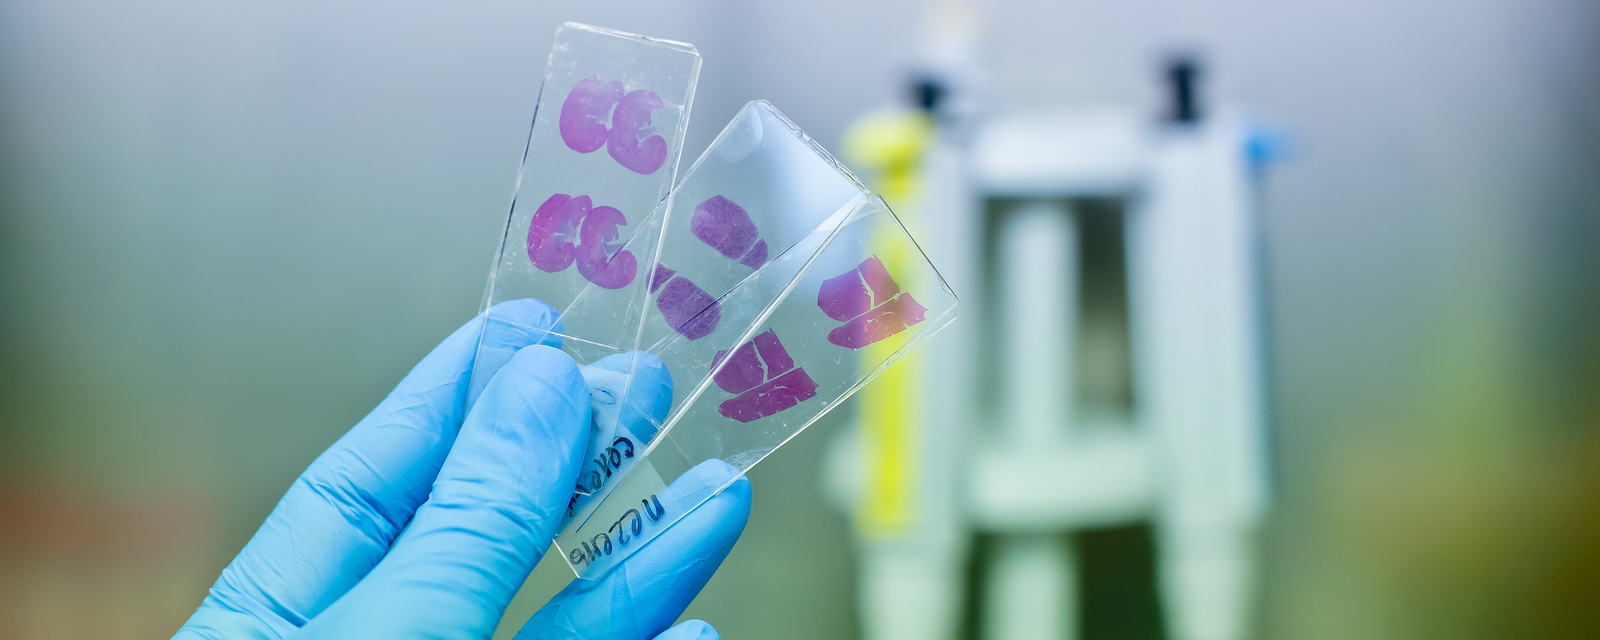
\includegraphics[width=1.0\textwidth,height=0.3\textheight]{figures/slide.jpg}
    \caption*{\label{fig:slide}}
  \end{figure}
  \vspace{-1.4cm}
  \begin{figure}[ht]
    \centering
    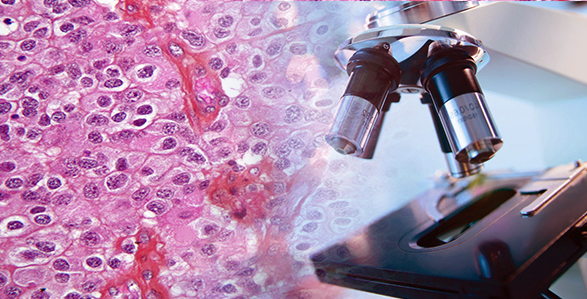
\includegraphics[width=1.0\textwidth,height=0.45\textheight]{figures/slide_microscope.jpg}
    \caption*{\label{fig:slide}}
  \end{figure}
\end{frame}
\begin{frame}
  \frametitle{Histology (cont'd)}
  Anatomic pathologists evaluate histology to classify and grade lesions
  \vspace{0.5cm}
  \begin{columns}[t]
    \begin{column}{.48\textwidth}
      Cancer diagnosis:
      \begin{itemize}
        \item characteristics
          \begin{itemize}
            \item nuclear atypia
            \item mitotic activity
            \item cellular density
            \item tissue architecture
          \end{itemize}
        \item incorporating
          \begin{itemize}
            \item cytologic details
            \item higher-order patterns
          \end{itemize}
      \end{itemize}
    \end{column}
    \begin{column}{.48\textwidth}
      Cancer prognostication:
      \begin{itemize}
        \item genomic biomarkers
          \begin{itemize}
            \item genetic alterations
            \item gene expression
            \item epigenetic modifications
          \end{itemize}
      \end{itemize}
    \end{column}
  \end{columns}
\end{frame}
\begin{frame}
  \frametitle{Time-to-Event Data Analysis}
  \begin{itemize}
    \item Logistic regression finds associations between risk factors and
    presence/absence of a disease
    \begin{itemize}
      \item we are interested in how a risk factor ortreatment affects time to disease or some other event
    \end{itemize}
  \end{itemize}
  bla bla bla\\

  Cox proportional hazard likelihood \\

  redicting survival using genomic profiles containing hundreds to tens of
  thousands of features (29, 30) and using basic clinical profiles containing 14
  features (31).

\end{frame}
\begin{frame}
  \frametitle{Survival Convolutional Neural Networks (SCNN)}
  prediction of time-to-event outcomes from histology images. \\
  SCNN framework uses an image sampling and risk filtering technique that
  significantly improves prediction accuracy by mitigating the effects of
  intratumoral heterogeneity and deficits in the availability of labeled data
  for training.
\end{frame}

\section{Methods}\label{sec:methods}
\begin{frame}
  \frametitle{Data and Image Curation}
  \begin{itemize}
    \item Brain cancer from TCGA (LGG and GBM cohorts)
    \item Removed images containing
    \begin{itemize}
      \item bubbles
      \item section folds
      \item pen markings
      \item poor (over or under) staining
      \item geographic necrosis
    \end{itemize}
    \item After filtering: 1,061 WSI from 769 unique patients
    \item ROI images (1,024 $\times$ 1,024) were cropped at 20$\times$
    \item Color-normalized to a gold standard H\&E calibration
    \item 256 $\times$ 256 patches were sampled from ROIs
    \item Randomized transformations applied to patches
    \begin{itemize}
      \item tissue orientation (mirror) and color variations (contrast and brightness)
    \end{itemize}
  \end{itemize}
\end{frame}
\begin{frame}
  \frametitle{VGG19 Architecture}
  \begin{figure}[ht]
    \centering
    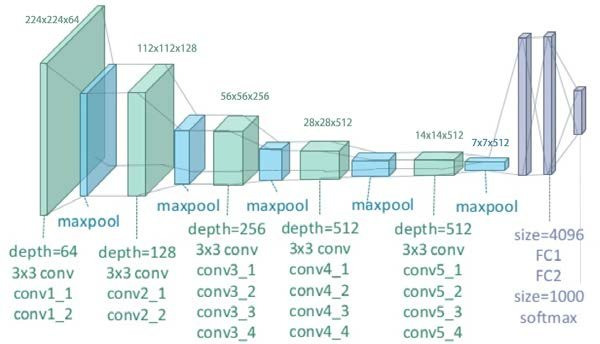
\includegraphics[width=1.0\textwidth,keepaspectratio]{figures/vgg19.jpg}
    \caption*{\label{fig:vgg19}}
  \end{figure}
\end{frame}
\begin{frame}
  \frametitle{Risk Prediction}
  $R=\beta^{T}X$
  \begin{itemize}
    \item $\beta \in \mathbb{R}^{256 \times 1}$ are weights
    \item $X \in \mathbb{R}^{256 \times 1}$ are inputs
    \item Backpropagation:
    $L(\beta, X)=-\sum_{i \in U}\left(\beta^{T} X_{i}-\log \sum_{j \in \Omega_{i}} e^{\beta^{T} X_{j}}\right)$
    \begin{itemize}
      \item $U$ is the set of right-censored samples
      \item $\Omega_{i}$ is the set of ``at-risk'' samples with event or follow-up times
      \item $\Omega_{i}=\left\{j | Y_{j} \geq Y_{i}\right\}$
      \item $Y_{i}$ is the last follow up time of patient $i$
    \end{itemize}
    \item Optimizer: Adagrad
    \begin{itemize}
      \item initial accumulator = 0.1
      \item initial learning rate = 0.001 (learning rate decay factor = 0.1)
      \item variance scaling method is used to initialize model weights
      \item decay rate = 4e-4
      \item 100 epochs
      \item Stochastic gradient training with minibatch size 14
      \item Randomized minibatches
      \item Regularization: Dropout in the last fully connected layer
    \end{itemize}
  \end{itemize}
\end{frame}
\begin{frame}
  \frametitle{Testing and Model Averaging}
  \begin{enumerate}
    \item $R_{m}^{j,k}$ denotes the risk of $k^{{\text{th}}}$ HPF in region $j$
    for patient $m$
    \item $R_{m}^{j}=\text{median}_{k}{\{R_{m}^{j,k}\}}$ (to reject outlying
    risks)
    \item $\widehat{R_{m}^{1}}>\widehat{R_{m}^{2}}>\widehat{R_{m}^{3}} \ldots$
    \item $R_{m}^{*}=\widehat{R_{m}^{2}}$
    \begin{itemize}
      \item robust to outliers or high risks that may occur due to some imaging or tissue-processing artifact
    \end{itemize}
    \item Model averaging: $\overline{R_{m}^{*}}=\frac{1}{5} \sum_{\gamma=96}^{100} R_{m(\gamma)}^{*}$
  \end{enumerate}
\end{frame}
\begin{frame}
  \frametitle{Model Performance}
  \begin{itemize}
    \item Monte Carlo cross-validation (15 times)
    \begin{itemize}
      \item 80\% training
      \item 20\% testing
    \end{itemize}
    \item Prediction accuracy was measured using Harrell's $c$ index
    \begin{itemize}
      \item concordance between predicted risk and actual survival for testing samples
    \end{itemize}
  \end{itemize}
\end{frame}
\section{Conclusion}\label{sec:conclusion}
\begin{frame}
  \frametitle{Questions}
  \begin{center}
    \Huge{Questions?}
  \end{center}
  \begin{figure}
    \centering
    
\includegraphics[width=0.5\textwidth,keepaspectratio]{figures/walter.jpg}
  \end{figure}
\end{frame}
\begin{frame}[allowframebreaks]
  \frametitle{References}
  \printbibliography{}
\end{frame}
\end{document}

%%% Local Variables:
%%% mode: latex
%%% TeX-master: t
%%% End:

\message{ !name(presentation.tex) !offset(-385) }
